\documentclass[10pt, a4paper,spanish]{article}
\usepackage[utf8]{inputenc}

\usepackage{lipsum} % Package to generate dummy text throughout this template
\usepackage{varwidth}
\usepackage{hyperref}
\usepackage{graphicx}

\usepackage[T1]{fontenc} % Use 8-bit encoding that has 256 glyphs
\usepackage{microtype} % Slightly tweak font spacing for aesthetics

\usepackage[hmarginratio=1:1,top=32mm,columnsep=20pt]{geometry} % Document margins
\usepackage[hang, small,labelfont=bf,up,textfont=it,up]{caption} % Custom captions under/above floats in tables or figures
\usepackage{booktabs} % Horizontal rules in tables
\usepackage{float} % Required for tables and figures in the multi-column environment - they need to be placed in specific locations with the [H] (e.g. \begin{table}[H])
\usepackage{hyperref} % For hyperlinks in the PDF

\usepackage{lettrine} % The lettrine is the first enlarged letter at the beginning of the text
\usepackage{paralist} % Used for the compactitem environment which makes bullet points with less space between them

\usepackage{abstract} % Allows abstract customization
\renewcommand{\abstractnamefont}{\normalfont\bfseries} % Set the "Abstract" text to bold
\renewcommand{\abstracttextfont}{\normalfont\small\itshape} % Set the abstract itself to small italic text

\usepackage{titlesec} % Allows customization of titles
\renewcommand\thesection{\Roman{section}} % Roman numerals for the sections
\renewcommand\thesubsection{\Roman{subsection}} % Roman numerals for subsections
\titleformat{\section}[block]{\large\scshape\centering}{\thesection.}{1em}{} % Change the look of the section titles
\titleformat{\subsection}[block]{\large}{\thesubsection.}{1em}{} % Change the look of the section titles
\usepackage{enumitem}

\usepackage{fancyhdr} % Headers and footers
\pagestyle{fancy} % All pages have headers and footers
\fancyhead{} % Blank out the default header
\fancyfoot{} % Blank out the default footer
\fancyhead[C]{ \today \ $\bullet$ ICO $\bullet$ Tutoría 1: Estrategias de resolución} % Custom header text
\fancyfoot[RO,LE]{\thepage} % Custom footer text

%----------------------------------------------------------------------------------------
%	TITLE SECTION
%----------------------------------------------------------------------------------------

\title{\vspace{-15mm}\fontsize{24pt}{10pt}\selectfont\textbf{Tutoría 1: Estrategias de resolución}} % Article title

\author{Sergio García Prado}
\date{\today}

%----------------------------------------------------------------------------------------

\begin{document}

	\maketitle % Insert title

	\thispagestyle{fancy} % All pages have headers and footers


%----------------------------------------------------------------------------------------
%	TEXT
%----------------------------------------------------------------------------------------

	\section{Cuestiones}

		\subsection{A qué tipo de búsqueda da lugar la estrategia de resolución lineal:}

			\begin{enumerate}[label=\Alph*)]
				\item \textbf{Primero en profundidad}
				\item Primero en anchura
				\item Ninguna de las anteriores
			\end{enumerate}

			\paragraph{}
			La estrategia de resolución lineal da lugar a una búsqueda primero en profundidad entre las cláusulas que forman la Base de Conocimiento. La causa está originada por la restricción que implica que una resolución debe estar formada por una cláusula cualquiera y la última resolvente obtenida. Esto hace que se genere una búsqueda primero en profundidad hacia la clausula vacía.


		\subsection{?`Es necesaria la presencia de una cláusula unitaria en un conjunto de cláusulas para que exista una refutación por entrada?}

			\paragraph{}
			\textbf{Si} que lo es. La demostración se puede llevar a cabo apoyandose en la equivalencia con la estrategia de resolución unitaria. Esta estrategia requiere que una de las cláusulas utilizadas en cada resolución sea unitaria, por lo tanto implica la necesidad de existencia de al menos una de las cláusulas del conjunto inicial sea unitaria.


	\newpage
	\section{Problemas}

		\subsection{Sea S el conjunto de cláusulas $ \{ P(x), \lnot P(A) \lor Q(A), P(x) \lor \lnot Q(x), \lnot P(x) \lor \lnot Q(x) \} $. ?`Es inconsistente el conjunto de cláusulas S? ?`Por qué?}

			\paragraph{}
			Para probar si el conjunto $S$ de cláusulas es inconsistente podemos apoyarnos en el teorema de completitud por entradas, puesto que todas las clausulas de $S$ son de Horn. Debido a su equivalencia con la estrategia de resolución unitaria este teorema también es válido con dicho mecanismo. Por lo tanto si conseguimos encontrar un conjunto de derivaciones utilizando todas las cláusulas del conjunto $S$ que nos lleven a cláusula vacía habremos demostrado la inconsistencia de $S$.

			Puesto que en este caso hemos llegado a la cláusula vacía podemos asegurar que \textbf{S es inconsistente}.

			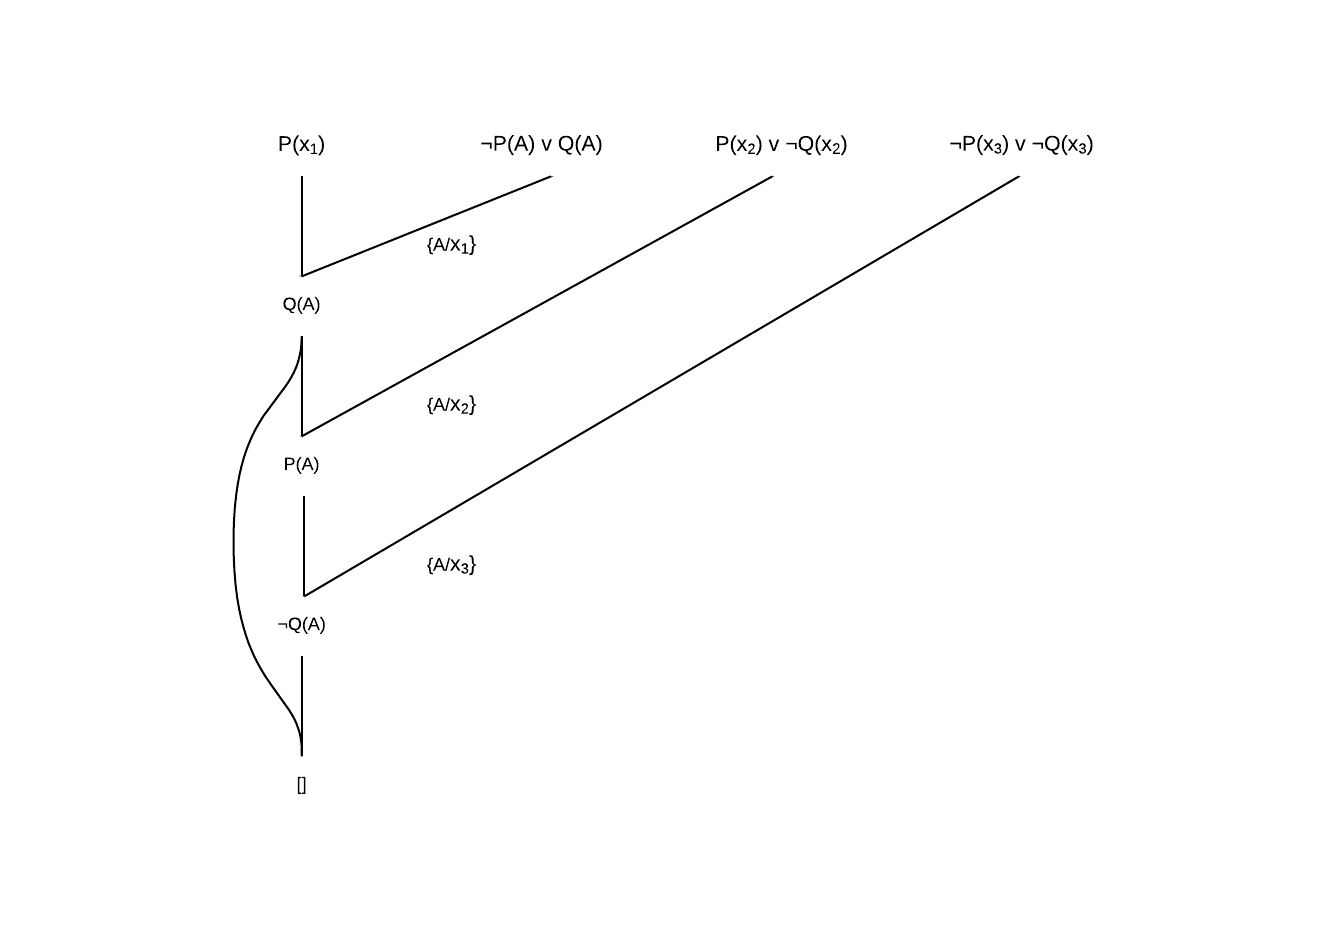
\includegraphics[width=\textwidth]{problem-1-resolution}


		\subsection{Sea S el conjunto de cláusulas $ \{ P(B), \lnot P(A) \lor Q(A), P(x) \lor \lnot Q(x), \lnot P(x) \lor \lnot Q(x) \} $. ?`Es inconsistente el conjunto de cláusulas S? ?`Por qué?}

			\paragraph{}
			Siguiendo el mismo razonamiento que en el ejercicio anterior, \textbf{$S$ no es inconsistente} dado que no podemos llegar a cláusula vacía mediante un conjunto de derivaciones, dado que existen dos constantes en el conjunto de cláusulas que lo impiden.


\end{document}
